\section{Mobile robot}
\subsection{Exercise 1}
The mobile robot considered in this assignment is represented by the schematics in figure \ref{fig:ex1_schematics}. 

\begin{figure}[H]
    \centering
    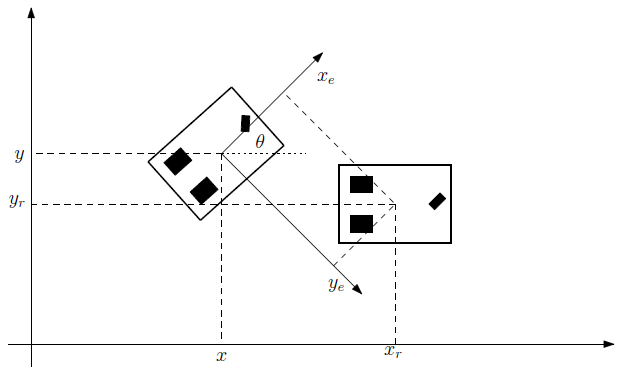
\includegraphics[width=0.7\textwidth]{Problems/ex1_schematic_system.PNG}
    \caption{Schematic representation system}
    \label{fig:ex1_schematics}
\end{figure}
It can be seen that there are reference coordinates represented in the figure by $x_r$ and $y_r$, actual coordinates represented by $x$, $y$ and $\theta$ and lastly error coordinates denoted by the subscript e. The kinematic model of the mobile robot is given by:

\begin{align}
    \dot{x} &= v \cos(\theta) \label{eq:ex1_kinmoda} \\
    \dot{y} &= v \sin (\theta) \label{eq:ex1_kinmodb}\\
    \dot{\theta} &= \omega \label{eq:ex1_kinmodc}
\end{align}
Where $v$ and $w$ are control inputs. The objective is to track a straight line with a constant velocity. These reference dynamics are given by:

\begin{align}
    \dot{x}_r &= v_r \cos(\theta_r) \label{eq:ex1_kinrefa}\\
    \dot{y}_r &= v_r \sin (\theta_r) \label{eq:ex1_kinrefb}\\
    \dot{\theta_r} &= \omega_r \label{eq:ex1_kinrefc}
\end{align}

The error coordinates can be written as a function of the actual and reference coordinates in the figure using the following transformation:
\begin{equation}
    \begin{bmatrix}
x_e\\ 
y_e\\
\theta_e

\end{bmatrix}
=
\begin{bmatrix}
\cos(\theta) & \sin(\theta)  & 0\\ 
-\sin(\theta) & \cos(\theta) & 0\\ 
0 & 0 & 1
\end{bmatrix}
\begin{bmatrix}
x_r - x\\
y_r - y\\
\theta_r - \theta 

\end{bmatrix}
\label{eq:ex1_error}
\end{equation}
A coordinate transformation is global if the transformation can be done in both directions for all coordinates. So the inverse of the transformation matrix should exist for all coordinates. By looking at the determinant of the matrix, it can be seen that the matrix is non-singular and therefore invertible. The determinant equals to: $\cos^2(\theta) + \sin^2(\theta)$. This is equal to 1 for every $\theta$. This means that the transformation is global, because the transformation matrix is always invertible. 

\subsection{Exercise 2}
In order to calculate the dynamics of the system represented in equation \eqref{eq:ex1_error}, the time derivative of this system should be computed. Using the product rule this results in the following:
\begin{equation}
    \begin{bmatrix}
    \dot{x}_e \\
    \dot{y}_e \\
    \dot{\theta}_e
    \end{bmatrix}
    =
    \begin{bmatrix}
    -\dot{\theta} \sin(\theta) & \dot{\theta} \cos(\theta) & 0 \\
    -\dot{\theta}\cos(\theta) & -\dot{\theta}\sin(\theta) & 0 \\
    0 & 0 & 0
    \end{bmatrix}
    \begin{bmatrix}
    x_r - x\\
    y_r - y\\
    \theta_r - \theta
    \end{bmatrix}
    +
    \begin{bmatrix}
    \cos(\theta) & \sin(\theta) & 0 \\
    -\sin(\theta) & \cos(\theta) & 0 \\
    0 & 0 & 1
    \end{bmatrix}
    \begin{bmatrix}
    \dot{x}_r - \dot{x}\\
    \dot{y}_r - \dot{y}\\
    \dot{\theta}_r - \dot{\theta}
    \end{bmatrix}
    \label{eq:ex2_dt}
\end{equation}
By expanding this and substituting the expressions from equations \eqref{eq:ex1_kinmoda} - \eqref{eq:ex1_kinrefc} and simplifying leads to the final error dynamics:
\begin{equation}
\begin{bmatrix}
\dot{x}_e \\
\dot{y}_e \\
\dot{\theta}_e
\end{bmatrix}
=
\begin{bmatrix}
\omega y_e - v + v_r \cos(\theta_e) \\
-\omega x_e + v_r \sin(\theta_e) \\
\omega_r - \omega
\end{bmatrix}
\label{eq:ex2_errordyn}
\end{equation}



\subsection{Exercise 3}

In order to stabilise the closed loop system, the control inputs $v$ and $\omega$ are chosen as:
\begin{align}
v &= v_r \cos(\theta_e) + \frac{k_1 x_e}{\sqrt{1+x_e^2 + y_e^2}} \label{eq:ex3_inputv}\\
\omega &= \omega_r + \frac{k_2 v_r y_e}{\sqrt{1 + x_e^2 + y_e^2}} + k_3 \sin(\theta_e) \label{eq:ex3_inputw}
\end{align}
In order to check the stability of the closed loop system, the following Lyapunov function is proposed:
\begin{equation}
    V(x_e, y_e, \theta_e) = -1 + \sqrt{1 + x_e^2 + y_e^2} + \frac{1}{k_2} ( 1 - \cos(\theta_e)
    \label{eq:ex3_lyap}
\end{equation}
This Lyapunov function is positive definite and can therefore be used to look at stability. This is done by taking the time derivative of the Lyapunov function. This time derivative can be written as:
\begin{equation}
    \dot{V}(x_e,y_e,\theta_e) = \frac{x_e \dot{x}_e + y_e \dot{y}_e}{\sqrt{1 + x_e^2 + y_e^2}} + \frac{\dot{\theta}_e}{k_2} \sin(\theta_e)
    \label{eq:ex3_lyapdtstep}
\end{equation}
This substitution and simplification this expression can be written in the form:
\begin{equation}
    \dot{V}(x_e, y_e, \theta_e) = -\frac{k_1 x_e^2}{1+x_e^2 + y_e^2} - \frac{k_3}{k_2} \sin^2(\theta_e)
    \label{eq:ex3_lyapdt}
\end{equation}
In order to asses asymptotic stability, the $\dot{V}$ should be negative definite. It can be seen that based on the properties of the variables in equation \eqref{eq:ex3_lyapdt} that \dot{V} is always smaller than zero if $x_e$ is not equal to zero and $\theta_e$ is not equal to $k \pi$. Using LaSalle's principle, asymptotic stability can still be guaranteed. $x_e = 0$ means that $\dot{x}_e = 0$. Using equation \eqref{eq:ex2_errordyn} this means that $\omega y_e - v + v_r \cos (\theta_e) = 0$. By substituting the control inputs from equation \eqref{eq:ex3_inputv} - \eqref{eq:ex3_inputw} and simplifying it can be seen that this is only the case for $x_e = 0$ and $y_e = 0$, which is in the equilibrium point. Furthermore $\theta_e = k \pi$ means that $\dot{\theta}_e = 0$ means that $\omega_r - \omega = 0$. Again, using substitution it can then be seen that this is only the case for $y_e = 0$ and $\theta_e = k \pi$. Since this is also the equilibrium point and using LaSalle's principle, the closed-loop system is asymptotically stable.

\subsection{Exercise 4}
In the feedback controller in equation \eqref{eq:ex3_inputv} and \eqref{eq:ex3_inputw} it can be seen that there is a term $\frac{k_1 x_e}{\sqrt{1 + x_e^2 + y_e^2}}$ and $\frac{k_2 v_r y_e}{\sqrt{1 + x_e^2 + y_e^2}}$ respectively. This makes the amplitude of these terms bounded by the gains $k_1$ and $k_2 v_r$. In order to further proof this, the extreme cases can be assessed. If $x_e$ becomes large and $y_e$ is zero, the term $\frac{k_1 x_e}{\sqrt{1 + x_e^2 + y_e^2}}$ is maximal and asymptotically go to $k_1$. This is desired, because a larger error should be corrected with a higher control gain. For the controller term $\omega$, the extreme case is when $y_e$ becomes large and $x_e$ is zero, the term $\frac{k_2 v_r y_e}{\sqrt{1 + x_e^2 + y_e^2}}$ is maximal and asymptotically goes to $k_2 v_r$. Which means that the gain depends on the reference velocity. The error in the angle between the mobile robot and the reference needs to be corrected with a higher gain if the velocity is bigger. So the ratio between the linear and the square root terms in the controller make sure that the controllers are bounded.




\subsection{Exercise 5}
In order to proof local around the equilibrium point $X_{eq} = (x_e, y_e, \theta_e = (0, 0, k\pi)$ Lyapunov's first method can be used. This is done by linearising. This is done using:

\begin{equation}
    \begin{bmatrix}
    \dot{z}_x \\ 
    \dot{z}_y \\ 
    \dot{z}_{\theta}
    \end{bmatrix}
    =
    F(X_{eq}) + \frac{\partial F}{\partial X} |_{X_{eq}} (Z - X_{eq})
    \label{eq:ex5_linear}
\end{equation}
Here, $F = \begin{bmatrix}
\dot{x}_e \\ \dot{y}_e \\ \dot{\theta}_e
\end{bmatrix}$ in equation \eqref{eq:ex2_errordyn}, $X = \begin{bmatrix}
x_e \\ y_e \\ \theta_e
\end{bmatrix}$ and $Z = \begin{bmatrix}
z_x \\ z_y \\ z_{\theta}
\end{bmatrix}$
This leads to the following linearized system after expanding, simplifying and using $\omega_r = 0$:
\begin{equation}
    \begin{bmatrix}
    \dot{z}_x \\ 
    \dot{z}_y \\ 
    \dot{z}_{\theta}
    \end{bmatrix}
    =
    A \begin{bmatrix}
    z_x \\ z_y \\ z_{\theta} -k \pi
    \end{bmatrix}
    =
    \begin{bmatrix}
    -k_1 & 0 & 0 \\
    0 & 0 & v_r \cos(\theta_e) \\
    0 & -k_3 v_r & -k_3 \cos(\theta_e)
    \end{bmatrix}
    \begin{bmatrix}
    z_x \\ z_y \\ z_{\theta} -k \pi
    \end{bmatrix}
    \label{eq:ex5_linear2}
\end{equation}
Where the eigenvalues of the $A$ matrix have to be determined in order to say something about local stability around $X_{eq}$. This leads to the following two cases, one where $\theta_e = 2 k \pi$ and one where $\theta_e = (2k + 1) \pi$. This leads to two sets of three eigenvalues: \\
If $\theta_e = 2 k \pi$:
\begin{align}
    \lambda_1 &= -\frac{1}{2} - \frac{1}{2} \sqrt{k_3^2 - 4 k_2 v_r^2} \label{eq:ex5_eigstablea} \\
    \lambda_2 &= -\frac{1}{2} + \frac{1}{2} \sqrt{k_3^2 - 4 k_2 v_r^2} \label{eq:ex5_eigstableb} \\
    \lambda_3 &= - k_1 \label{eq:ex5_eigstablec}
\end{align}
All these eigenvalues are smaller than zero, because $k_1$, $k_2$, $k_3$ and $v_r^2$ are all bigger than zero. For the other case, where $\theta_e = (2k + 1)\pi$, the following set of eigenvalues is computed:
\begin{align}
    \lambda_1 &= -\frac{1}{2} - \frac{1}{2} \sqrt{k_3^2 + 4 k_2 v_r^2} \\
    \lambda_2 &= -\frac{1}{2} + \frac{1}{2} \sqrt{k_3^2 + 4 k_2 v_r^2} \\
    \lambda_3 &= - k_1    
\end{align}
All these eigenvalues are not smaller than zero using the same reasoning as before. \\
It can therefore be concluded that the system is locally stable around the equilibrium point if $\theta_e = 2 k \pi$, because the eigenvalues are all smaller than zero and locally unstable if $\theta_e = (2k + 1) \pi$, because not all eigenvalues are smaller than zero.
\subsection{Exercise 6}
In equation \eqref{eq:ex5_eigstablea} - \eqref{eq:ex5_eigstablec} the stable eigenvalues can be seen. The eigenvalues all be placed at -1 by computing $k_1$, $k_2$ and $k_3$ accordingly. This leads to $k_1 = 1$, $k_2 = 2$ and $k_3 = \frac{1}{2}$. Using an ode45 solver in matlab, the system can be simulated for a straight line as a reference which can be written as:

\begin{equation}
    (x_r, y_r, \theta_r, v_r, \omega_r) = (t, t, \frac{\pi}{4}, \sqrt{2}, 0).
\end{equation}
This is done for the following initial conditions:
\begin{itemize}
    \item ($x_0, y_0, \theta_0$) = ($-30, -21, \frac{\pi}{4}$)
    \item ($x_0, y_0, \theta_0$) = ($0, 0, \pi$)
    \item ($x_0, y_0, \theta_0$) = ($0, 1, -\frac{\pi}{4}$)
\end{itemize}
The results for the three initial conditions can be seen below:
\subsubsection*{Initial conditions ($x_0, y_0, \theta_0$) = ($-30, -21, \frac{\pi}{4}$)}
\begin{figure}[H]
\begin{minipage}{0.5\textwidth}
    \centering
    \includegraphics[width=\textwidth]{Problems/ex6_errora.eps}
    \caption{Error dynamics simulation results for ($x_0, y_0, \theta_0$) = ($-30, -21, \frac{\pi}{4}$)}
    \label{fig:ex6_errora}
\end{minipage}
\begin{minipage}{0.5\textwidth}
    \centering
    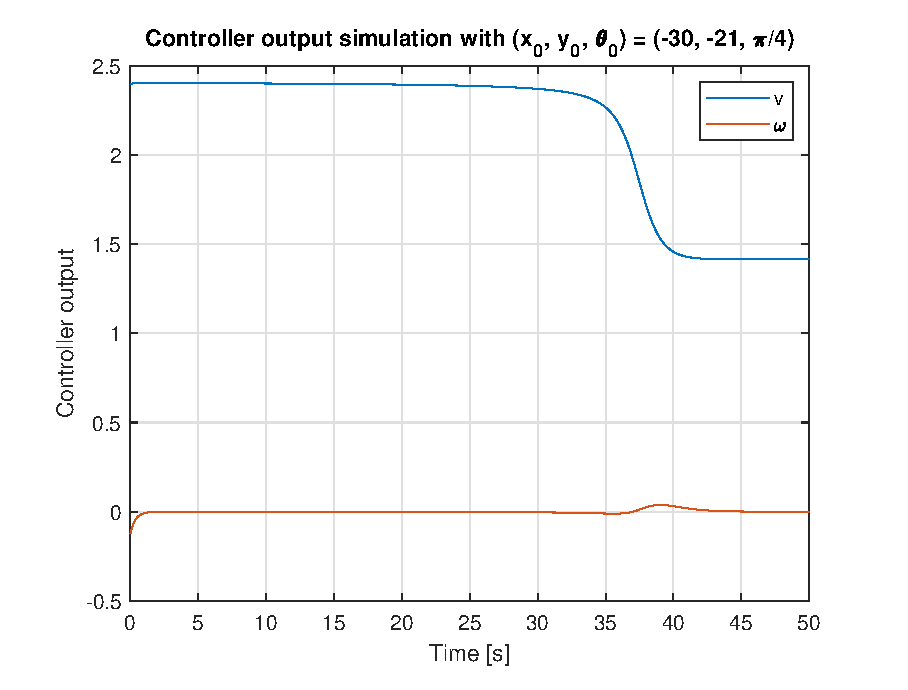
\includegraphics[width=\textwidth]{Problems/ex6_controla.eps}
    \caption{Control output simulation results for ($x_0, y_0, \theta_0$) = ($-30, -21, \frac{\pi}{4}$)}
    \label{fig:ex6_controla}
\end{minipage}
\end{figure}

As can be seen in figure \ref{fig:ex6_errora}, the error dynamics go towards zero. This is desired, because that means that the mobile robot is tending towards the reference path. In the control output in figure \ref{fig:ex6_controla}, the trailer will first drive towards the reference line with a higher velocity, when it arrives at the reference line, the trailer will steer in order to drive in the same direction as the reference line and the control output $v$ will go to $v_r = \sqrt{2}$. 


\subsubsection*{Initial conditions ($x_0, y_0, \theta_0$) = ($0, 0, \pi$)}
\begin{figure}[H]
\begin{minipage}{0.5\textwidth}
    \centering
    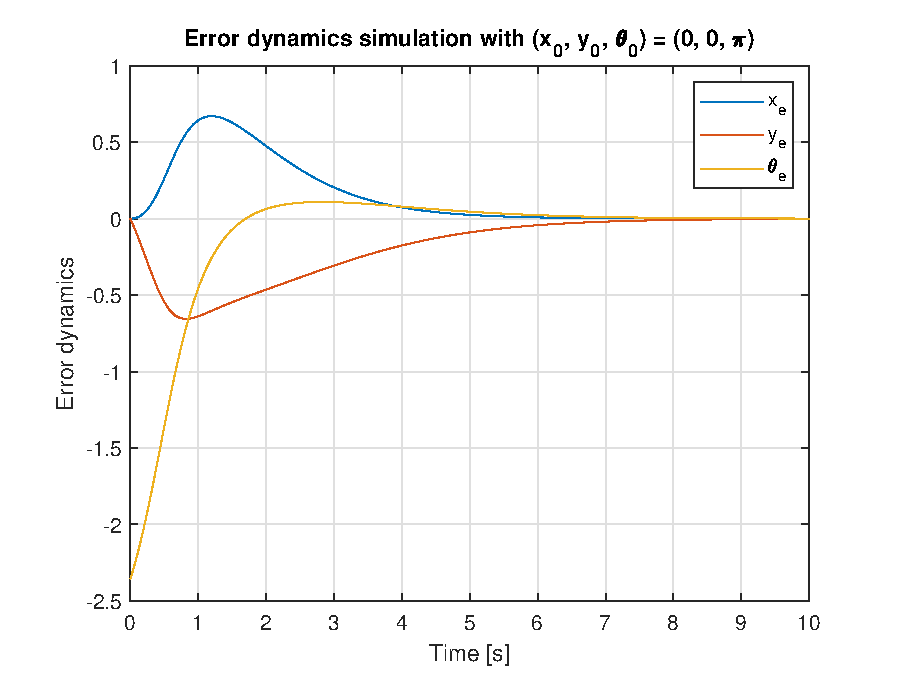
\includegraphics[width=\textwidth]{Problems/ex6_errorb.eps}
    \caption{Error dynamics simulation results for ($x_0, y_0, \theta_0$) = ($0, 0, \pi$)}
    \label{fig:ex6_errorb}
\end{minipage}
\begin{minipage}{0.5\textwidth}
    \centering
    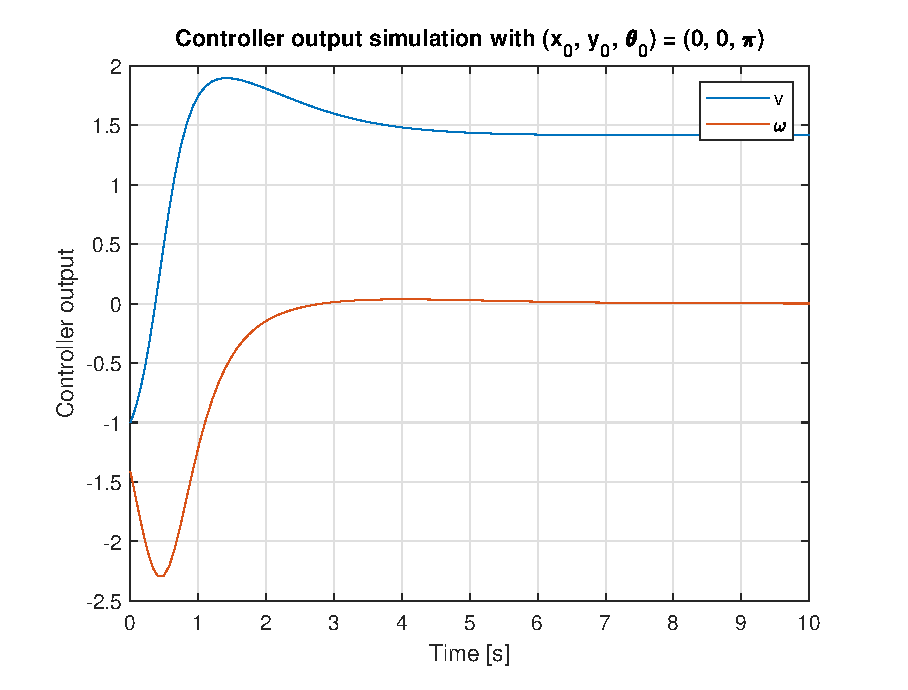
\includegraphics[width=\textwidth]{Problems/ex6_controlb.eps}
    \caption{Control output simulation results for ($x_0, y_0, \theta_0$) = ($0, 0, \pi$)}
    \label{fig:ex6_controlb}
\end{minipage}
\end{figure}

There is only an error in the angle initially. This first results in an error in the $x$ and $y$ coordinate, which is compensated for by the control input. It can be seen that the error goes towards zero and $v$ and $\omega$ go towards $v_r = \sqrt{2}$ and $\omega_r = 0$ respectively.

\subsubsection*{Initial conditions ($x_0, y_0, \theta_0$) = ($0, 1, -\frac{\pi}{4}$)}
\begin{figure}[H]
\begin{minipage}{0.5\textwidth}
    \centering
    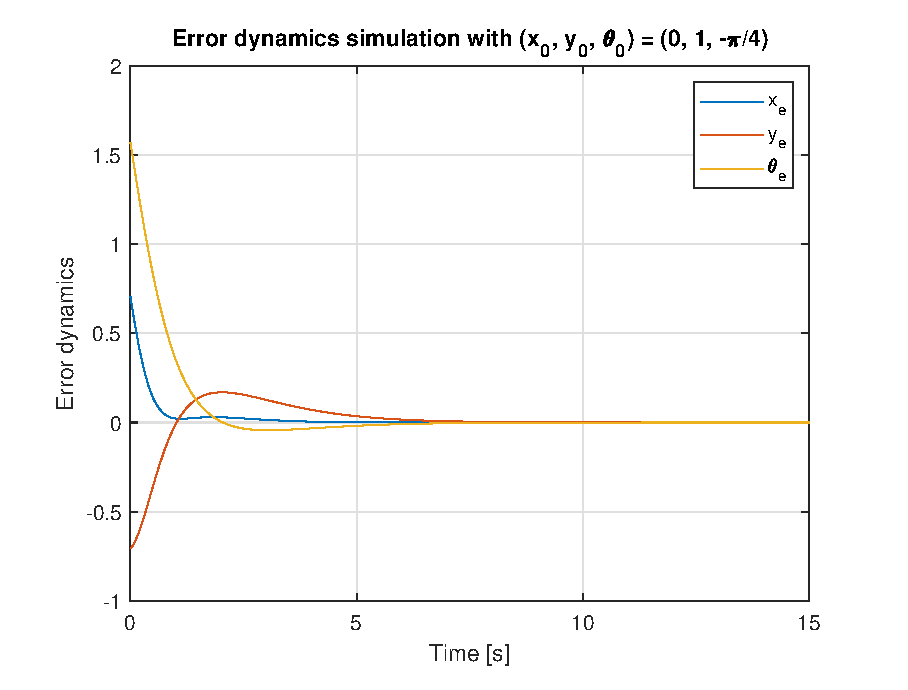
\includegraphics[width=\textwidth]{Problems/ex6_errorc.eps}
    \caption{Error dynamics simulation results for ($x_0, y_0, \theta_0$) = ($0, 1, -\frac{\pi}{4}$)}
    \label{fig:ex6_errorc}
\end{minipage}
\begin{minipage}{0.5\textwidth}
    \centering
    \includegraphics[width=\textwidth]{Problems/ex6_controlc.eps}
    \caption{Control output simulation results for ($x_0, y_0, \theta_0$) = ($0, 1, -\frac{\pi}{4}$)}
    \label{fig:ex6_controlc}
\end{minipage}
\end{figure}

For the last initial conditions, there is only an error in $y$ coordinate as can be seen in figure \ref{fig:ex6_errorb}. Since the mobile robot can not move in the that direction purely, an error in the $x$ coordinate is a result of compensating for that error. The mobile robot will again steer in the direction of the reference line. The control output $v$ will again go towards $v_r = \sqrt{2}$. The control output $\omega$ will go to $\omega_r = 0$ as can be seen in figure \ref{fig:ex6_controlb}.

\subsection{Exercise 7}

Now a trailer attached to the mobile robot will be considered. This can be seen in the schematic representation below:

\begin{figure}[H]
    \centering
    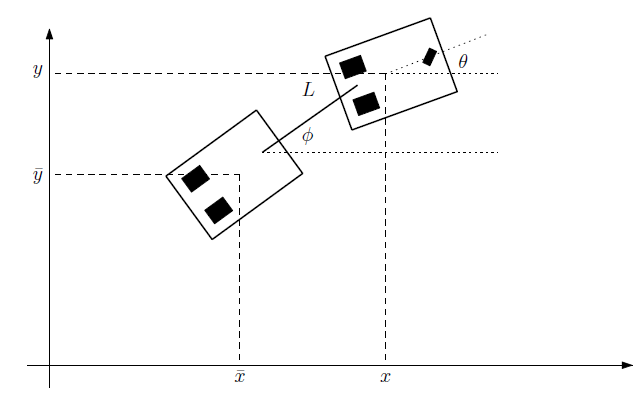
\includegraphics[width=0.7\textwidth]{Problems/ex7_schematic_system.PNG}
    \caption{Schematic representation system with trailer}
    \label{fig:ex7_schematics}
\end{figure}

The kinematic equations of the mobile robot will remain the same as in equations \eqref{eq:ex1_kinmoda} - \eqref{eq:ex1_kinmodc}. The addition of the trailer results in additional kinematics which describe the dynamics of the trailer with respect to the mobile robot:
\begin{equation}
    \dot{\phi} = \frac{v}{L} \sin(\theta - \phi)
    \label{eq:ex7_trailerdyn}
\end{equation}
Where $\phi$ is the angle between the trailer and the $x$-axis indicated in figure \ref{fig:ex7_schematics}. The total dynamics of the system can be described as following:
\begin{equation}
    \begin{bmatrix}
    \dot{x} \\
    \dot{y} \\
    \dot{\theta} \\
    \dot{\phi} 
    \end{bmatrix}
    =
    \begin{bmatrix}
    v \cos(\theta) \\
    v \sin(\theta) \\
    \omega \\
    \frac{v}{L} \sin(\theta - \phi)
    \end{bmatrix}
    \label{eq:ex7_robottrailerdyn}
\end{equation}
It is again the objective to track a certain reference with the following dynamics:
\begin{equation}
    \begin{bmatrix}
    \dot{x}_r \\
    \dot{y}_r \\
    \dot{\theta}_r \\
    \dot{\phi}_r
    \end{bmatrix}
    =
    \begin{bmatrix}
    v_r \cos(\theta) \\
    v_r \sin(\theta) \\
    \omega_r \\
    \frac{v_r}{L} \sin(\theta_r - \phi_r)
    \end{bmatrix}
    \label{eq:ex7_robottrailerrefden}
\end{equation}

The same coordinate transformation as in equation \eqref{eq:ex1_error} can be used and expanded using $\phi_e = \phi_r - \phi$ for the addition of the trailer and can be written as:
\begin{equation}
    \begin{bmatrix}
    x_e \\
    y_e \\
    \theta_e \\
    \phi_e
    \end{bmatrix}
    =
    \begin{bmatrix}
    \cos(\theta) & \sin(\theta) & 0 & 0 \\
    -\sin(\theta) & \cos(\theta) & 0 & 0 \\
    0 & 0 & 1 & 0 \\
    0 & 0 & 0 & 1
    \end{bmatrix}
    \label{eq:ex7_error}
\end{equation}
Using the same approach as in exercise 2, with the use of the chain rule and simplifying this, the error dynamics can written as:
\begin{equation}
    \begin{bmatrix}
    \dot{x}_e \\
    \dot{y}_e \\
    \dot{\theta}_e \\
    \dot{\phi}_e
    \end{bmatrix}
    =
    \begin{bmatrix}
    \omega y_e - v + v_r \cos(\theta_e) \\
    -\omega x_e + v_r \sin(\theta_e) \\
    \omega_r - \omega \\
    \frac{v_r}{L} \sin(\theta_r - \phi_r) - \frac{v}{L} \sin(\theta - \phi)
    \end{bmatrix}
    \label{eq:ex7_errordyn}
\end{equation}


\subsection{Exercise 8}

The remaining error dynamics (zero-dynamics) of the system in equation \eqref{eq:ex7_errordyn} can be determined by using $x_e\;=\;y_e\;=\;\theta_e\;=\;
0$, $v\;=\;v_r$ and $\omega\;=\;\omega_r\;=\;0$. This will result in:
\begin{equation}
    \begin{bmatrix}
    \dot{x}_e \\
    \dot{y}_e \\
    \dot{\theta}_e \\
    \dot{\phi}_e
    \end{bmatrix}
    =
    \begin{bmatrix}
    0 \\
    0 \\
    0 \\
    - \frac{v}{L}\sin(\phi_e)
    \end{bmatrix}
    \label{eq:ex8_zero}
\end{equation}
So there is only zero-dynamics for the $\dot{\phi}_e$. It can be seen that if $v_r>0$, the dynamics are stable if $\phi_e\;=\;2 k \pi$, since a positive $\phi_e$ results in negative dynamics $\dot{\phi}_e$ and vice versa. For $v_r < 0$ the zero-dynamics are stable for $\phi_e\;=\;(2k + 1) \pi$, because then the same holds as described before.


\section{Backstepping}


\subsection{Exercise 9}
In the previous exercises the mobile robot with trailer had to track a certain reference trajectory, from now on a controller is designed that ensures that the attached trailer tracks a certain reference trajectory. For this a new coordinate frame for the trailer is defined

\begin{align}
\overline{x} &= x - L \cos{\phi} \label{eq:ex9_trailercoords_a}\\
\overline{y} &= y - L \sin{\phi} \label{eq:ex9_trailercoords_b}\\
\overline{\theta} &= \phi,
\label{eq:ex9_trailercoords_c}
\end{align}

which represent the position ($\overline{x}$,$\overline{y}$) and orientation $\overline{\theta}$ of the trailer. The kinematic model of the trailer is given by

\begin{align}
    \dot{\overline{x}} &= \overline{v} \cos{\overline{\theta}} \label{eq:ex9_trailerkinematic_a}\\
    \dot{\overline{y}} &= \overline{v} \sin{\overline{\theta}} \label{eq:ex9_trailerkinematic_b}\\
    \dot{\overline{\theta}} &= \overline{\omega},
    \label{eq:ex9_trailerkinematic_c}
\end{align}

where

\begin{align}
    \overline{v} &= v\cos(\theta-\overline{\theta}) \label{eq:ex9_trailerinput_v}\\
    \overline{\omega} &= \frac{v}{L}\sin(\theta-\overline{\theta}).
    \label{eq:ex9_trailerinput_w}
\end{align}

Similarly to equations \eqref{eq:ex1_kinrefa} - \eqref{eq:ex1_kinrefc}, a reference can be specified for the trailer, and the error coordinates can be specified in a similar way as to equation \eqref{eq:ex1_error}. This results in the following tracking error dynamics

\begin{align}
    \dot{\overline{x}}_e &= \overline{\omega}\overline{y}_e - \overline{v} + \overline{v}_r\cos\overline{\theta}_e \label{eq:ex9_error_a} \\
    \dot{\overline{y}}_e &= -\overline{\omega} \overline{x}_e  + \overline{v}_r\sin\overline{\theta}_e \label{eq:ex9_error_b} \\
    \dot{\overline{\theta}}_e &= \overline{\omega}_r - \omega \label{eq:ex9_error_c}.
\end{align}

These dynamics have a similar structure as in equations \eqref{eq:ex2_errordyn}, so based on the previously calculated controller in exercise 3 it can be concluded that choosing 

\begin{align}
    \overline{v} &= \overline{v}_r\cos\overline{\theta}_e + \frac{k_1\overline{x}_e}{\sqrt{1+\overline{x}^2_e+\overline{y}^2_e}} \label{eq:ex9_virtualinput_v}\\
    \overline{\omega} &= \overline{\omega}_r + \frac{k_2\overline{y}_e\overline{v}_r}{\sqrt{1+\overline{x}^2_e+\overline{y}^2_e}} + k_3\sin\overline{\theta}_e \label{eq:ex9_virtualinput_w}
\end{align}

stabilises the trailer dynamics when the gains $k_i > 0$, $i$ = 1,2,3. However $\overline{v}, \overline{\omega}$ are virtual inputs which stabilise the trailer dynamics at $(\overline{x}_e,\overline{y}_e,\overline{\theta}_e) = (0,0,k\pi)$. Rewriting the virtual input $\overline{v}$ into the real input $v$ using equation \eqref{eq:ex9_trailerinput_v} results in 

\begin{equation}
    v = \frac{\overline{v}}{\cos(\theta-\overline{\theta})} = \frac{\overline{v}_r\cos\overline{\theta}_e + \frac{k_1\overline{x}_e}{\sqrt{1+\overline{x}^2_e+\overline{y}^2_e}}}{\cos(\theta-\overline{\theta})}. \label{eq:ex9_input_v}\\
\end{equation}

Rewriting equation \eqref{eq:ex9_trailerinput_w} in the same form as done in equation \eqref{eq:ex9_input_v} and filling in the the expressions for $v$ and $\overline{\omega}$ with the assumption that $\overline{\omega}_r = 0$ results in the equation

\begin{equation}
    \frac{\overline{v}_r\cos\overline{\theta}_e + \frac{k_1\overline{x}_e}{\sqrt{1+\overline{x}^2_e+\overline{y}^2_e}}}{\cos(\theta-\overline{\theta})} = \frac{\frac{L k_2 \overline{y}_e \overline{v}_r}{\sqrt{1+\overline{x}^2_e+\overline{y}^2_e}} + L k_3 \sin\overline{\theta}_e}{\sin(\theta-\overline{\theta})}. \label{eq:ex9_psicalc}
\end{equation}

Introducing a new virtual input $\psi := \tan(\theta-\overline{\theta})$, and rewriting equation \eqref{eq:ex9_psicalc} results in an expression for $\psi$

\begin{equation}
    \psi = L \Big( \frac{k_2\overline{y}_e\overline{v}_r + k_3 \sqrt{1+\overline{x}_e^2+\overline{y}_e^2}\sin\overline{\theta}_e}{k_1\overline{x}_e + \overline{v}_r\sqrt{1+\overline{x}_e^2+\overline{y}_e^2}\cos\overline{\theta}_e} \Big). \label{eq:ex9_psi}
\end{equation}

Because this is essence only a coordinate transform from ($\overline{v}, \overline{\omega}$) to ($v, \psi$) the stability of the tracking error dynamics remains unchanged, and thus equations \eqref{eq:ex9_input_v} and \eqref{eq:ex9_psi} stabilise the system given by equations \eqref{eq:ex9_error_a} - \eqref{eq:ex9_error_c} at the points $(\overline{x}_e,\overline{y}_e,\overline{\theta}_e) = (0,0,k\pi)$.



\subsection{Exercise 10}
Next the error dynamics of the trailer is extended to include the error between the virtual input $\psi$ and the desired virtual input $\psi_d$. This new error is therefor defined as $\psi_e := \psi - \psi_d$. Where the expression given in equation \eqref{eq:ex9_psi} defines $\psi_d$ resulting in

\begin{equation}
    \psi_e = \tan(\theta-\overline{\theta}) - L \Big( \frac{k_2\overline{y}_e\overline{v}_r + k_3 \sqrt{1+\overline{x}_e^2+\overline{y}_e^2}\sin\overline{\theta}_e}{k_1\overline{x}_e + \overline{v}_r\sqrt{1+\overline{x}_e^2+\overline{y}_e^2}\cos\overline{\theta}_e} \Big). \label{eq:ex10_psi_e}
\end{equation}

Of which the dynamics are given by taking the derivative resulting in
\begin{equation}
    \dot{\psi}_e = \dot{\psi} - \dot{\psi}_d, \label{eq:ex10_psiedot}
\end{equation}

with
\begin{equation}
    \dot{\psi} = (\omega - \overline{\omega})(\psi^2 + 1). \label{eq:ex10_psidot}
\end{equation}

The term $\dot{\psi}_d$ was calculated using the symbolic toolbox in matlab. The expression is very long and will therefore not be given in this report. It is however used for the computations and simulations.
\subsection{Exercise 11}
Using backstepping to design a controller for $\omega$ that stabilises the error dynamics, the fist step is to define new coordinates for the error dynamics and write the error dynamics in these new coordinates. So the new coordinates are chosen to be

\begin{align}
    z_1 &= \overline{x}_e \label{eq:ex11_newcoordsz_1} \\
    z_2 &= \overline{y}_e \label{eq:ex11_newcoordsz_2} \\
    z_3 &= \overline{\theta}_e \label{eq:ex11_newcoordsz_3} \\
    z_4 &= \overline{\psi}_e  = \psi - \psi_d \label{eq:ex11_newcoordsz_4}.
\end{align}

This than results in the error dynamics becoming

\begin{align}
    \dot{z}_1 &= \frac{\overline{v}}{L}z_2(z_4+\psi_d) - \overline{v} + \overline{v}_r\cos z_3 \label{eq:ex11_dynz_1} \\
    \dot{z}_2 &= -\frac{\overline{v}}{L}z_1(z_4+\psi_d) + \overline{v}_r\sin z_3 \label{eq:ex11_dynz_2}\\
    \dot{z}_3 &= \overline{\omega}_r - \frac{\overline{v}_r}{L}(z_4+\psi_d) \label{eq:ex11_dynz_3} \\
    \dot{z}_4 &= \Big(\omega - \frac{\overline{v}}{L}(z_4+\psi_d)\Big)\Big((z_4+\psi_d)^2+1\Big)-\dot{\psi}_d \label{eq:ex11_dynz_4},
\end{align}

when using 

\begin{equation}
    \overline{\omega} = \frac{\overline{v}}{L}\psi = \frac{\overline{v}}{L}(z_4+\psi_d). \label{eq:ex11_omegabar}
\end{equation}

Equation \eqref{eq:ex11_omegabar} is derived from substituting equation \eqref{eq:ex9_trailerinput_v} into equation \eqref{eq:ex9_trailerinput_w}. Choosing $\omega$ in such a way that $\dot{\psi}_e = u$ resulting in 

\begin{equation}
    \omega = \frac{\overline{v}}{L}(z_4+\psi_d) + \frac{\dot{\psi}_d + u}{(z_4+\psi_d)^2+1}. \label{eq:ex11_omega}
\end{equation}

Than using the Lyapunov function 

\begin{equation}
    V = -1 + \sqrt{1+z_1^2+z_2^2} + \frac{1}{k_2}(1-\cos z_3) + \frac{1}{2}z_4^2 \label{eq:ex11_lyap}
\end{equation}

to find a $u$ that stabilises the system. This is done by taking the derivative and cancelling all non-negative terms and subtracting $z_4$, resulting in 

\begin{equation}
    u = \frac{\frac{1}{2}\overline{v}_r\sin(2z_3)(1+z_1^2+z_2^2)+k_1z_1\sqrt{1+z_1^2+z_2^2}\sin z_3}{L k_2(1+z_1^2+z_2^2)} - z_4 \label{eq:ex11_u}
\end{equation}

Substituting this back into $\omega$ results in the final stabilising controller for the system given by equations \eqref{eq:ex9_error_a} - \eqref{eq:ex9_error_c} and \eqref{eq:ex10_psiedot}, with equilibrium points $(\overline{x}_e,\overline{y}_e,\overline{\theta}_e,\psi_e) = (0,0,k\pi,0)$. This means that the mobile robot is able to drive forwards and backwards with the trailer in a straight line. Because the system tends towards a situation where in the trailer is following a straight reference line due to the equilibrium points of $\overline{x}_e,\overline{y}_e,\overline{\theta}_e$ and the trailer stays in line with the cart because of $\psi_e = 0$.

\subsection{Exercise 12}
The following $A$-matrix is considered for the system:
\begin{equation}
    A = \begin{bmatrix}
    0 & 1 & 0 \\
    0 & 0 & 1 \\
    -k_1 & -k_2 & -k_3
    \end{bmatrix}
    \label{eq:ex12_A}
\end{equation}

In order to get the eigenvalues of this matrix at -1, the function acker in matlab can be used. To use acker in matlab however, an $A'$-matrix and $B$-vector is needed. That can be done by splitting the matrix in to the following:
\begin{align}
    A' &= \begin{bmatrix}
    0 & 1 & 0\\
    0 & 0 & 1 \\
    0 & 0 & 0
    \end{bmatrix} \\
    B &= \begin{bmatrix}
    0 \\ 0 \\ 1
    \end{bmatrix}
\end{align}
Satisfying $A\;=\;A'\;+\;BK$ with $K \;= \; \begin{bmatrix} k_1 & k_2 & k_3 \end{bmatrix} ^T $
Now with acker the poles can be placed at -1. This results in $k_1\;=\;1$, $k_2\;=\;3$ and $k_3\;=\;3$. The system was simulated using an ode45 solver and the resulting dynamics of the mobile robot and the trailer can be seen in figure \ref{fig:ex12_dyn}. The position of the mobile robot and the trailer are also plotted in the xy-plane, which can be seen in figure \ref{fig:ex12_xyposition}.

\begin{figure}[H]
\begin{minipage}{0.5\textwidth}
    \centering
    \includegraphics[width=\textwidth]{Problems/ex12_dynamics.eps}
    \caption{Dynamics system mobile robot with trailer}
    \label{fig:ex12_dyn}
\end{minipage}
\begin{minipage}{0.5\textwidth}
    \centering
    \includegraphics[width=\textwidth]{Problems/ex12_xyposition.eps}
    \caption{Position of mobile robot with trailer in x-y-plane}
    \label{fig:ex12_xyposition}
\end{minipage}
\end{figure}
It can be seen in figure \ref{fig:ex12_dyn} that the x and y coordinate of both the mobile robot and the trailer are changing linearly over time, both with the same slope, which is because of the angle of $\pi/4$. The angle of the mobile robot and the trailer are also similar and approximately equal to $\pi/4$. In the beginning there steering is happening and the angle of the mobile robot and the trailer are changing a little bit. This can also be seen in the plot in figure \ref{fig:ex12}. The mobile robot and the trailer are going over the same line, but the mobile robot a length of $\frac{sqrt{2}}{2}$ behind the cart. This can also be seen by the fact that the mobile robot does not start in at the same place in figure \ref{fig:ex12_xyposition} on the top right. 
\subsection{Exercise 13}


\section{Input-output linearisation}

\subsection{Exercise 14}

The tracking dynamics are again considered as:

\begin{align}
    \dot{x}_e &= \omega y_e + v_r (\cos(\theta_e) -1) \label{eq:ex14_dotx}\\
    \dot{y}_e &= \omega x_e + v_r \sin(\theta_e) \label{eq:ex14_doty}\\
    \dot{\theta}_e &= \omega - \omega_r \label{eq:ex14_dottheta}\\
    \dot{\phi}_e &= \frac{v_r}{L}\sin(\theta_e - \phi_e) \label{eq:ex14_dotphi}
\end{align}

Now $v\;=\;v_r\;<\;0$ and only $\omega$ as an input. The output is defined as $q\;=\;\phi_e$. The relative degree can be determined by taking the time derivative of the output and looking at what derivative the input appears. So the output is as follows:
\begin{equation}
    q = \phi_e
    \label{eq:ex14_q}
\end{equation}
The time derivative of the output will be:
\begin{equation}
    \dot{q} = \dot{\phi}_e = \frac{v_r}{L}\sin(\theta_e - \phi_e)
    \label{eq:ex14_qdot}
\end{equation}
Finally, the second time derivative of the output is:
\begin{equation}
    \Ddot{q} = \frac{v_r}{L} \cos(\theta_e - \phi_e) ( \omega - \omega_r - \frac{v_r}{L} \sin(\theta_e - \phi_e))
    \label{eq:ex14_qddot}
\end{equation}
It can be seen that the input appears in the second time derivative of the output. This means that the relative degree of the system is equal to 2. This is well defined if $\cos(\theta_e - \phi_e)\;\neq\;0$. So when $\theta_e - \phi_e\;\neq\;(k + \frac{1}{2}) \pi$.


\subsection{Exercise 15}

The input/output behaviour can be linearized by choosing the input in a clever way. The input will be written in the following form:
\begin{equation}
    \omega = \alpha(x_e, y_e, \theta_e, \phi_e) + \beta(x_e, y_e, \theta_e, \phi_e) u
    \label{eq:ex15_w}
\end{equation}
Where $u$ is an new virtual input that should be chosen in a way that the linearized input/output behaviour is stable. The input can be written as:

\begin{equation}
    \omega = (L_g L_f^{k-1} h(x))^{-1} (-L_f^k h(x) + u)
    \label{eq:ex15_w1}
\end{equation}

Filling this in and expanding leads to:
\begin{equation}
    \omega = \frac{\frac{v_r}{L}\cos(\theta_e - \phi_e)(\omega_r + \frac{v_r}{L}\sin(\theta_e - \phi_e)) + u}{\frac{v_r}{L} \cos(\theta_e - \phi_e)}
    \label{eq:ex15_w2}
\end{equation}
By comparing equation \eqref{eq:ex15_w} with equation \eqref{eq:ex15_w2}, $\alpha$ and $\beta$ can be determined:
\begin{align}
    \alpha(x_e, y_e, \theta_e, \phi_e) &= \omega_r + \frac{v_r}{L}\sin(\theta_e - \phi_e) \label{eq:ex15_alpha} \\
    \beta(x_e, y_e, \theta_e, \phi_e) &= \frac{1}{\frac{v_r}{L} \cos(\theta_e - \phi_e)}
\end{align}
By choosing $\omega$ in that way, the second time derivative of the output will equal the new virtual input: $\Ddot{q} = u$. In order to stabilise the input/output behaviour the following expression for the virtual input can be used to converge to a certain desired output $q_d$:
\begin{equation}
    u = -a_1 \dot{q} - a_0 (q - q_d)
    \label{eq:ex15_u}
\end{equation}
The eigenvalues of this should be in the open left-half plane in order to ensure stability. The following equation should be solved:
\begin{equation}
    \lambda^2 + a_1 \lambda + a_0 = 0
    \label{eq:ex15_eigvaleq}
\end{equation}

Has the following eigenvalues:
\begin{align}
    \lambda_1 = \frac{-a_1 + \sqrt{a_1^2 - 4a_0}}{2} \label{eq:ex15_lam1} \\
    \lambda_2 = \frac{-a_1 - \sqrt{a_1^2 - 4a_0}}{2} \label{eq:ex15_lam2} 
\end{align}

Both eigenvalues are chosen to be equal to -1, this results in $a_1\;=\;2$, $a_0\;=\;1$, which means that the following is a stabilizing controller with poles at -1:

\begin{equation}
    u = -2 \dot{q} - (q - q_d)
    \label{eq:ex15_contr}
\end{equation}

\subsection{Exercise 16}

To conclude on stability of the zero-dynamics, the system in equations \eqref{eq:ex14_dotx} - \eqref{eq:ex14_dotphi} have to be analysed. For zero-dynamics, perfect tracking has to be considered. This means that $\theta_e \; = \; \phi_e \; = \; k \pi$, $\omega \; = \; \omega_r \; = \; 0$. Substituting this in equations \eqref{eq:ex14_dotx} - \eqref{eq:ex14_dotphi} results in the following:
\begin{equation}
    \begin{bmatrix}
    \dot{x}_e \\
    \dot{y}_e \\
    \dot{\theta}_e \\
    \dot{\phi}_e
    \end{bmatrix}
    =
    \begin{bmatrix}
    v_r (\cos(\theta_e) - 1) \\
    0 \\
    0 \\
    0
    \end{bmatrix}
    \label{eq:ex16_zero}
\end{equation}
Using that $\theta_e \; = \; k\pi$, it stable if $\cos(\theta_e) \; = \; 1$, because then $\dot{x}_e \; = \; 0$ and the system is unstable if $\cos(\theta_e) \; = \; -1$, because then $\dot{x}_e \; = \; -2*v_r$. This means that the system is stable for $\theta_e \; = \; 2 k \pi$ and unstable for $\theta_e \; = \; (2+1)k\pi$


